\documentclass[journal ]{new-aiaa}
%\documentclass[conf]{new-aiaa} for conference papers
\usepackage[utf8]{inputenc}
\usepackage{textcomp}

\usepackage{graphicx}
\usepackage{amsmath}
\usepackage[version=4]{mhchem}
\usepackage{siunitx}
\usepackage{longtable,tabularx}
\usepackage{mylistingstyle}
\usepackage{longtable}
\setlength\LTleft{0pt} 

\title{Place a good Title for Image Preprocessing Framework Here}

\author{Author: Luis Kraker\footnote{BsC, Master's student in System Test Engineering, FH-Joanneum}}
\affil{FH-Joanneum, Graz 8020, Austria}
\author{Supervisor: Mrs. Gudrun Schappacher Tilp\footnote{DDr, Associate Professor at FH-Joanneum}}
\affil{FH-Joanneum, Graz 8020, Austria}

\begin{document}

\maketitle

\begin{abstract}
	Make The beautiful abstract here.
\end{abstract}



\section{Introduction}
\lettrine{T}{he} field of computer vision is increasingly prevalent; it is a powerful tool in the industry and offers a wide range of applications, including multimedia, robotics, manufacturing, medicine, and autonomous driving.\cite{bebis2002review}
Central to these applications is image preprocessing, which prepares images for subsequent analysis and feature extraction. Effective image preprocessing enhances image quality, facilitates the extraction of relevant features, and accelerates the entire machine learning pipeline.\cite{gonzalez2002digital}\cite{nelson2020image}\cite{krig2014image}

Despite the importance of image preprocessing, using popular libraries like TensorFlow (\cite{tensorflow2015}) and OpenCV (\cite{opencv2000}) often presents challenges:
\begin{itemize}
    \item Experimentation with different techniques or parameters is cumbersome due to scattered code.
    \item Reproducibility is hindered by the lack of straightforward methods to save and load preprocessing pipelines.
    \item Lack of modularity makes the code tightly coupled with the rest of the codebase, complicating maintenance and updates.
    \item Integrating preprocessing routines with various machine learning frameworks often requires duplicating code.
    \item The complexity of existing solutions can be daunting for beginners.
\end{itemize}

To overcome these challenges, we propose a simple, modular image preprocessing framework that offers high-level abstractions for common preprocessing tasks. Built on OpenCV and TensorFlow, this framework provides a user-friendly API that facilitates experimentation, ensures reproducibility through easy pipeline management, allows for automatic experimantation and enhances modularity for better integration with diverse machine learning environments. This paper details the design and implementation of our framework and demonstrates its application in a typical computer vision task.



\section{Implementation}
The image preprocessing framework is developed using Python, leveraging the capabilities of TensorFlow and OpenCV. TensorFlow, a robust machine learning library, provides extensive end-to-end machine learning tools and computational efficiency, allowing for the integration of complex machine learning functionalities. OpenCV is used for its advanced image processing capabilities, offering a range of operations that are not available in TensorFlow, thus enriching the framework's processing abilities.

\subsection{Framework Overview}
Inspired by the scikit-learn's Pipeline design, our framework enables chaining multiple image processing steps into a cohesive pipeline, specifically tailored for image data. Unlike scikit-learn, which is generally used for tabular data, our framework focuses exclusively on image preprocessing without extending into model training.

The primary objective of the framework is to simplify and streamline the image preprocessing pipeline for computer vision tasks. Specifically, it aims to:
\begin{itemize}
    \item Enable easy chaining of multiple image processing steps.
    \item Facilitate the application of these steps to complete datasets efficiently.
    \item Allow for straightforward randomization of pipeline configurations, beneficial for hyperparameter optimization.
    \item Provide simple mechanisms for saving and loading pipelines, enhancing reproducibility and ease of experimentation.
    \item Ensure the framework is easily extendable with new image processing steps, accommodating evolving requirements and new techniques.
\end{itemize}

\subsection{Framework Architecture}
\label{sec:framework_architecture}
The framework consists of several key classes that drive its functionality:
\begin{itemize}
    \item \texttt{ImagePreprocessor} class serves as the central component of the framework. It manages the configuration and execution of the image preprocessing pipeline.
    \item \texttt{StepBase} class acts as an abstract base class for all preprocessing steps, ensuring consistency and providing common functionalities.
    \item \texttt{ClassInstancesSerializer} utility class provides methods for serializing and deserializing the pipeline configurations, facilitating reproducibility and experimentation.
    \item \texttt{Preprocessing Steps} encapsulate specific preprocessing operations within subclasses of \texttt{StepBase}, enhancing the framework's modularity.
\end{itemize}

The Unified Modeling Language (UML) diagram in Figure~\ref{fig:framework_uml} illustrates the relationships between these classes and their public methods.

\newpage
\begin{figure}[h]
    \centering
    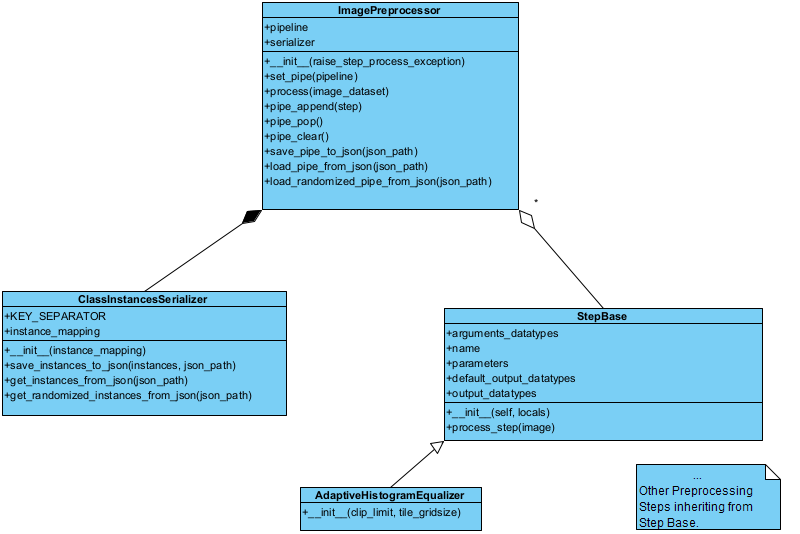
\includegraphics[width=0.8\textwidth]{image_preprocessing_uml.png}
    \caption{UML Diagram of the Image Preprocessing Framework}
    \label{fig:framework_uml}
\end{figure}


\subsection{Preprocessing Operations}
Each preprocessing operation is encapsulated within a subclass of \texttt{StepBase}, implementing specific functionalities such as adaptive histogram equalization. These classes enhance the framework's modularity, allowing users to easily customize and extend the pipeline. Listing ~\ref{lst:preprocessing_step} demonstrates the implementation of an adaptive histogram equalization step, that can be seamlessly integrated into the preprocessing pipeline. The example showcases the simplicity and straightforwardness of adding new preprocessing steps to the framework.\\

\begin{lstlisting}[language=Python, caption=Example of a Preprocessing Step Implementation, label=lst:preprocessing_step]
class AdaptiveHistogramEqualizer(StepBase):
    arguments_datatype = {'clip_limit': float, 'tile_gridsize': (int, int)}
    name = 'Adaptive Histogram Equalizer'

    def __init__(self, clip_limit=2.0, tile_gridsize=(8,8)):
        super().__init__(locals())

    @StepBase._nparray_pyfunc_wrapper
    def process_step(self, image_nparray):
        channels = cv2.split(image_nparray)
        clahe = cv2.createCLAHE(clipLimit=self.parameters['clip_limit'],
                                tileGridSize=self.parameters['tile_gridsize'])
        clahe_channels = [clahe.apply(ch) for ch in channels]
        clahe_image = cv2.merge(clahe_channels)
        return clahe_image
\end{lstlisting}

\subsection{Serialization and Deserialization}
The framework offers a straightforward method for serializing and deserializing the preprocessing pipeline configuration, facilitated by the \texttt{ClassInstancesSerializer} class. This class handles the conversion of the pipeline configuration into a JSON format and back, taking advantage of JSON's readability, editability, and hierarchical organization, which suits the pipeline's structure well. The \texttt{ClassInstancesSerializer} also manages the datatypes of the pipeline parameters to ensure they are compatible with JSON formatting. It is responsible for transforming the parameters of the preprocessing steps into a format that can be serialized in JSON and for restoring the original datatypes upon deserialization. When creating a preprocessing step class, one needs to specify the datatypes of the parameters in the \texttt{arguments\_datatype} class variable. The \texttt{ImagePreprocessor} class, in conjunction with the \texttt{ClassInstancesSerializer}, handles the serialization and deserialization processes.


\subsection{Testing Strategies of the Framework}
The robustness of our framework is guaranteed through a comprehensive testing approach utilizing Python's \texttt{unittest} module. Each core class within the framework, as outlined in Section \ref{sec:framework_architecture}, is equipped with its own suite of tests. These tests encompass both unit tests, which scrutinize the functionality of individual methods, and integration tests, which assess the interactions between classes to ensure cohesive operation.

To maintain consistency across the preprocessing steps and avoid duplicative testing efforts, we have developed a unified test suite. This suite is specifically designed to validate the implementation of preprocessing steps and their seamless integration within the framework. It is systematically applied to all preprocessing components to confirm compliance with established standards and to prevent the introduction of errors.

Furthermore, we have implemented a rigorous test scenario known as the "long pipeline test." This test is critical for evaluating the framework's capacity to manage extensive preprocessing pipelines. It involves applying multiple, lengthy pipelines—comprising a significant number of preprocessing steps—to a diverse set of images. The sequence of steps within these pipelines is randomized to confirm the framework's ability to handle various configurations effectively. This test is pivotal in ensuring that even the most complex preprocessing pipelines are processed efficiently and correctly by the framework.


\section{Application}
The Image Preprocessing framework facilitates a straightforward and intuitive process for setting up and applying image preprocessing pipelines.

\subsection{Setting Up the Preprocessing Pipeline}
The steps to configure the preprocessing pipeline are outlined below:

\begin{enumerate}
    \item Instanciate the \texttt{ImagePreprocessor} class.
    \item Construct the preprocessing pipeline by specifying the sequence of desired preprocessing steps.
    \item Set the configured pipeline to the \texttt{ImagePreprocessor} instance.
    \item Finally, apply the pipeline to the image dataset for processing.
\end{enumerate}
This procedure is illustrated in Listing~\ref{lst:application_example}.
\begin{lstlisting}[language=Python, caption=Example of Applying the Image Preprocessing Pipeline, label=lst:application_example]
# Initialize the Image Preprocessor
preprocessor = ImagePreprocessor()

# Define the Preprocessing Pipeline
pipeline = [
    steps.AdaptiveHistogramEqualizer(clip_limit=4.0, tile_gridsize=[4, 4]),
    steps.ShapeResizer(desired_shape=[1500, 1500], resize_method='bilinear'),
    steps.RGBToGrayscale(),
    steps.BinaryThresholder(thresh=128),
    steps.Mirrorer(mirror_direction='horizontal'),
]

# Set the Pipeline 
preprocessor.set_pipe(pipeline)

# Apply the Pipeline to the Dataset
processed_dataset = preprocessor.process(image_dataset)
\end{lstlisting}

\subsection{Visualizing Preprocessing Results}
The effects of the preprocessing pipeline are visually demonstrated in Figure~\ref{fig:preprocessing_results}, which compares images from the PCB Defect Dataset before and after preprocessing.

\begin{figure}[h]
    \centering
    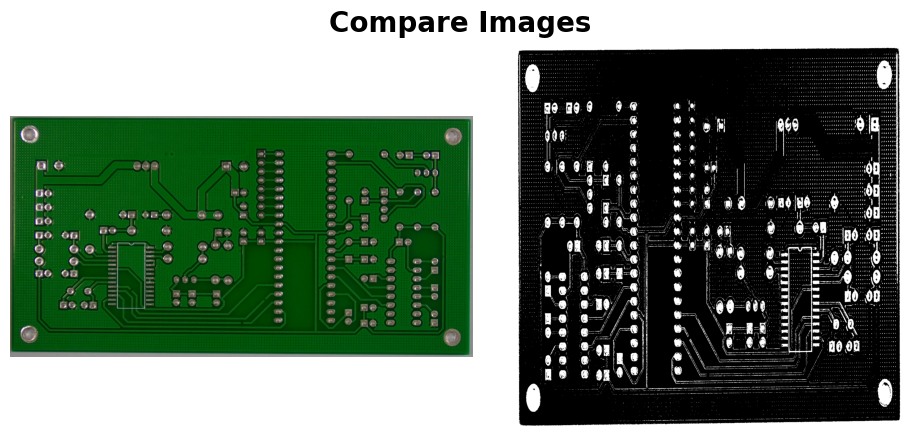
\includegraphics[width=0.8\textwidth]{preprocessing_results.png}
    \caption{Preprocessing Results of the Image Preprocessing Pipeline}
    \label{fig:preprocessing_results}
\end{figure}

\subsection{Overview of Implemented Preprocessing Operations}
A summary of the currently implemented preprocessing operations, categorized by their types, is provided in the following table:

\begin{longtable}{|p{0.3\linewidth}|p{0.65\linewidth}|}
    \hline
    \textbf{Category} & \textbf{Preprocessing Steps} \\
    \hline
    \endhead
    \hline
    \endfoot
    
    \textbf{Histogram Equalization} & Adaptive Histogram Equalizer, Global Histogram Equalizer \\
    \hline
    \textbf{Blurring \& Smoothing} & Gaussian Blur Filter, Median Blur Filter, Bilateral Filter, Average Blur Filter \\
    \hline
    \textbf{Thresholding} & Otsu Thresholding, Adaptive Thresholding, Binary Thresholding, Truncated Thresholding, Threshold to Zero \\
    \hline
    \textbf{Noise Reduction \& Injection} & Non Local Mean Denoiser, Gaussian Noise Injector \\
    \hline
    \textbf{Color Space Conversion} & RGB To Grayscale, Grayscale To RGB \\
    \hline
    \textbf{Geometric Transformations} & Rotator, Mirrorer, Shape Resizer, Square Shape Padder \\
    \hline
    \textbf{Morphological Operations} & Erosion Filter, Dilation Filter, Dilate Erode Sequencer \\
    \hline
    \textbf{Normalization} & Min Max Normalizer, Standard Normalizer, Mean Normalizer, Local Contrast Normalizer \\
    \hline
    \textbf{Random Augmentations} & Random Color Jitterer, Random Sharpening, Random Rotator, Random Flipper, Random Cropper, Random Perspective Transformer, Random Elastic Transformer \\
    \textbf{Miscellaneous} & TypeCaster, Clipper, Scaler \\
    \hline
\end{longtable}

\subsection{Randomization of the Preprocessing Pipeline}
The framework offers a method to randomize the configurations of the preprocessing pipeline, which is useful for exploring the effects of different preprocessing settings on image datasets. This functionality is particularly beneficial for hyperparameter optimization and various experimental scenarios. Users can specify potential values or distributions for each parameter within the JSON configuration, and the framework will randomly select from these options during the application of the pipeline.


\section{Discussion}
The Image Preprocessing Framework is specifically tailored to work with TensorFlow's image dataset format. This limitation stems from the decision to harness TensorFlow's computational efficiencies for managing the pipeline's processing. Despite this restriction, the framework's design facilitates a user-friendly, modular, and extensible environment that supports a wide array of preprocessing operations through the integration of TensorFlow and OpenCV.

It is important to note that the framework does not include capabilities for learning or optimizing the parameters of preprocessing steps automatically. Instead, it focuses solely on preprocessing tasks to prepare data for subsequent model training, without encompassing model training itself. This delineation ensures that the framework remains streamlined and efficient for its designated preprocessing functions.

Moreover, the framework's architecture is crafted to emphasize simplicity, reproducibility, and modularity. These attributes ensure that users can easily experiment with different preprocessing configurations and seamlessly integrate the framework into diverse machine learning environments. One of the significant features of the framework is its support for the randomization of pipeline configurations, which greatly aids in hyperparameter optimization. This feature enhances the flexibility of the framework, permitting users to effectively explore and optimize preprocessing steps to suit specific requirements.

Overall, the framework offers a robust solution for managing image preprocessing pipelines, albeit within the constraints of the TensorFlow ecosystem. Its design also accommodates the straightforward addition of new preprocessing operations, allowing for continuous improvement and adaptation to new challenges and advancements in the field of image processing.



\section*{Acknowledgments}
Good Acknowledgments here.

\bibliography{sample}

\end{document}
